\documentclass[12pt,a4paper]{article}

\usepackage{fontawesome5}
\providecommand{\faPencilAlt}{\faIcon{pencil-alt}}

\usepackage{styles/couleurs}
\usepackage{styles/mise_en_page}
\usepackage{styles/boites}
\usepackage{styles/maths}
\usepackage{styles/figures}

\usepackage{enumitem}
\usepackage{array}
\usepackage{tabularx}
\usepackage{amsmath}
\usepackage{amssymb}
\usepackage{tikz}
\usepackage{xparse}

\usetikzlibrary{calc,angles,quotes,arrows.meta}

\setlist[itemize]{leftmargin=1.4em,itemsep=0.15em,topsep=0.2em}
\setlist[enumerate]{leftmargin=*,itemsep=0.22em,topsep=0.25em}

\newcommand{\lignepointillee}{\noindent\dotfill\par\vspace{0.45em}}

\newcommand{\lignesreponse}[1]{%
\begin{tcolorbox}[
enhanced,colback=white,colframe=NeutreC!40,boxrule=0.5pt,arc=1.5mm,
left=3mm,right=3mm,top=2mm,bottom=1mm,before skip=2pt,after skip=2pt]
\foreach \i in {1,...,#1}{\lignepointillee}
\end{tcolorbox}}

\newcommand{\titreseq}[1]{%
\begin{center}
{\sffamily\LARGE\bfseries\color{TitreC}Séquence 6 -- Cosinus d'un angle aigu}\\[0.2em]
{\sffamily\large\bfseries\color{SavoirC}#1}
\end{center}}

\begin{document}

\titreseq{Activité 3 -- Lire la figure et utiliser la calculatrice}

\section*{Partie A -- Le côté adjacent dépend de l'angle étudié}

\begin{center}
\begin{tikzpicture}[scale=1]
  \coordinate (A) at (0,0);
  \coordinate (B) at (4.8,0);
  \coordinate (C) at (4.8,3.2);

  \draw[line width=0.9pt] (A)--(B)--(C)--cycle;
  \draw (4.45,0)--(4.45,0.35)--(4.8,0.35);

  \node[left] at (A) {$A$};
  \node[below] at (B) {$B$};
  \node[above] at (C) {$C$};

  \draw[ActionC,line width=1pt] (0.75,0) arc[start angle=0,end angle=34,radius=0.75];
  \draw[SavoirC,line width=1pt] (4.8,2.45) arc[start angle=-90,end angle=-146,radius=0.75];

  \node[ActionC] at (1.08,0.38) {$\widehat A$};
  \node[SavoirC] at (4.35,2.2) {$\widehat C$};
\end{tikzpicture}
\end{center}

Complète.

\[
\text{Hypoténuse du triangle }ABC : \dotfill
\]

\[
\text{Côté adjacent à }\widehat A : \dotfill
\]

\[
\text{Côté adjacent à }\widehat C : \dotfill
\]

Explique pourquoi l'hypoténuse n'est jamais appelée « côté adjacent ».

\lignesreponse{4}

\section*{Partie B -- Le triangle choisi est essentiel}

Dans la figure, \(EGF\) est rectangle en \(F\), \(H\) appartient à \([EG]\)
et \(FH\) est perpendiculaire à \((EG)\).

\begin{center}
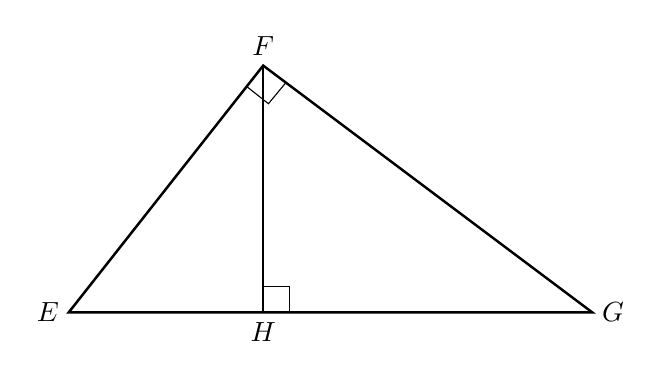
\begin{tikzpicture}[scale=0.95]
  \coordinate (E) at (0,0);
  \coordinate (G) at (7,0);
  \coordinate (F) at (2.6,3.3);
  \coordinate (H) at (2.6,0);

  \draw[line width=0.9pt] (E)--(F)--(G)--cycle;
  \draw[line width=0.9pt] (F)--(H);

  \draw (2.38,3.02)--(2.67,2.79)--(2.91,3.08);
  \draw (2.6,0.35)--(2.95,0.35)--(2.95,0);

  \node[left] at (E) {$E$};
  \node[above] at (F) {$F$};
  \node[right] at (G) {$G$};
  \node[below] at (H) {$H$};
\end{tikzpicture}
\end{center}

Complète.

\[
\text{Dans }EGF\text{ rectangle en }F,\qquad
\cos(\widehat{FEG})=\frac{\ldots}{\ldots}
\]

\[
\text{Dans }EHF\text{ rectangle en }H,\qquad
\cos(\widehat{FEH})=\frac{\ldots}{\ldots}
\]

\[
\text{Dans }GHF\text{ rectangle en }H,\qquad
\cos(\widehat{FGH})=\frac{\ldots}{\ldots}
\]

Que montre cet exemple sur la nécessité de nommer le triangle utilisé ?

\lignesreponse{4}

\section*{Partie C -- Définition}

\begin{tcolorbox}[colback=SavoirC!5,colframe=SavoirC!60,boxrule=0.7pt,arc=2mm]
Dans un triangle rectangle :

\[
\cos(\text{angle aigu})
=
\frac{\text{longueur du côté adjacent à cet angle}}
     {\text{longueur de l'hypoténuse}}.
\]

On peut aussi lire le quotient en ligne :

\[
\cos(\text{angle aigu})
=
\text{adjacent}\div\text{hypoténuse}.
\]
\end{tcolorbox}

\section*{Partie D -- La calculatrice}

Vérifie que la calculatrice est en \textbf{mode degré}, puis complète
au millième.

\[
\cos(20^\circ)\approx\ldots
\qquad
\cos(40^\circ)\approx\ldots
\]

\[
\cos(60^\circ)=\ldots
\qquad
\cos(80^\circ)\approx\ldots
\]

\begin{enumerate}
  \item Les valeurs sont-elles comprises entre \(0\) et \(1\) ?
  \item Lorsque l'angle aigu augmente, que semble faire son cosinus ?
  \item Pourquoi un cosinus n'est-il pas une longueur ?
\end{enumerate}

\lignesreponse{5}

\aretenir{Le cosinus est un nombre sans unité.
Pour un angle aigu, il est strictement compris entre \(0\) et \(1\).}

\end{document}
